\section{Background}

While our insight and approach is general, in order to demonstrate its
practicality we prototype it in the context of Clover~\cite{clover}, a
disaggregated key/value store.  Hence, we begin with a brief overview
of the relevant aspects of Clover's design for the uninitiated.

\subsection{Append-only updates}

\begin{figure}
    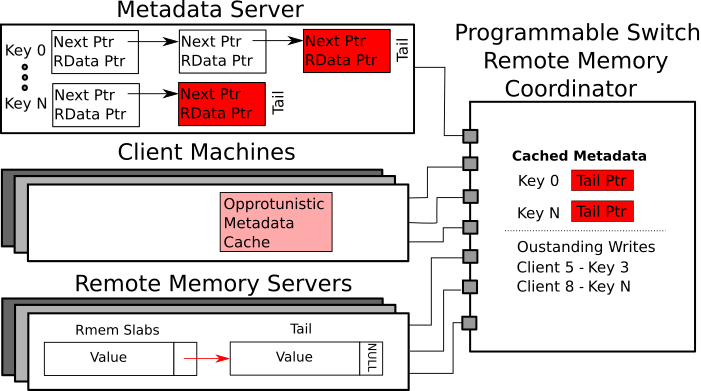
\includegraphics[width=0.45\textwidth]{fig/overview_2.png}
%%
    \caption{ System overview, Metadata, client, and Remote Memory
    servers are Clover components. Our remote memory coordinator is
    located on a centralized TOR interconnecting the clover components.
    }
%%
    \label{fig:overview} 
\end{figure}

Clover maximizes performance by storing data in a versioned list, dubbed a
\emph{chain} by the authors, which allows for fully asynchronous non-blocking
reads and $O(1)$ writes which succeed opportunistically. Writes are issued by
clients as atomic append operations to the end of the chain, the structure of
which is illustrated in Figure~\ref{fig:overview}. Each entry in the chain
contains a pointer to the next entry with the pointer at the tail of the
chain set to \texttt{NULL}. Clients keep cached pointers to the current tail of the
chain for each key allowing them to issue locf-free RDMA reads directly to

passive remote memory servers using the address they believe to be the
current tail. Clients can independently confirm their reads are
fresh by ensuring the value returned has a \texttt{NULL} next-update pointer.

Write (i.e., append-to-tail) operations, on the other hand, require two steps
in the common case. First a writer issues a lock-free RDMA write to store the
new value update to an uncontended portion of remote memory. The
second operation optimistically attempts to make the update globally visible
by atomically committing it to the end of the chain. Specifically, the writer
issues an RDMA compare-and-swap (\texttt{c\&s}) operation to the old tail to replace
its (presumably still \texttt{NULL}) next-update pointer with the address of the
new value. If successful, it then updates the metadata sever with
the new end-of-chain address.
%(as any concurrent writes to the same location will fail the comparison).

%% This operation ensures that the next
%% write to the data structure writes to the tail of the linked list.
%% This operation requires two steps.

The Clover authors compare their opportunistic approach with a variety
of different system architectures including one which centralizes
metadata on the datapath (pDPM-central). They find that their
opportunistic approach achieves extremely high throughput on
read-heavy workloads, performing similarly to raw RDMA reads.  In
contrast pDPM-central bottlenecks at far lower throughput.  In the
presence of writes Clover's throughput decreases due to contention
while the performance of pDPM-central remains the same as it resolves all
concurrent write conflicts in the data path.



\subsection{Conflict handling}

If multiple clients attempt to update the value concurrently, each will
succeed in their first write to their private region of remote memory but
then issue conflicting RDMA \texttt{c\&s} operations to the end of the shared chain.
The race is resolved at the remote memory location of the previous update in
the chain: only the first \texttt{c\&s} operation will succeed; all subsequent
operations will fail because rather than finding a value with a \texttt{NULL}
next-update pointer, they find the now (at best) penultimate value in the
chain which points to the update issued by the client that won the race.
%When concurrent writes update the same key a race occurs to write at the end
%of the chain. Write operations require two separate RDMA transactions that
%must each complete to ensure atomicity.
During this two-RTT operation any concurrent write to the same key will cause
a conflict.

%% The process which lost the race now needs to engage in \textit{Pointer
%% chasing} to find the new tail. It must iterative issue reads of the
%% linked list, step by step until it finds the location of the new tail.


If a client's write---or read---fails because it used a stale tail pointer
the client concurrently requests the new tail address from the metadata
server and iteratively traverses the chain themselves to find the current end
in a processes known as \emph{chain walking}. (It is insufficient to just
consult the metadata server because it is updated lazily.) Failed writers
must then issue a new \texttt{c\&s} operation at the updated end of the chain to
append their pending update. Of course, the reissued \texttt{c\&s} is subject to the
same race condition as many writers may be executing concurrently. This
pointer-chasing reconciliation algorithm must be run independently each time
a conflict occurs.
%The slower writers will fail the guard, and must retry their c\&s operation
%after walking the chain through remote memory or by getting an update from
%the metadata server.
While concurrent read operations will not prevent a write from succeeding, a
reader that loses the race with a \texttt{c\&s} operation will need to issue another
RDMA read to the new address to obtain the updated value. On write-heavy
workloads these race conditions happen frequently
%as illustrated in Figure~\ref{fig:conflicts}, , which leads to a sharp
%decrease in throughput. For highly contested structures, the number of
%retries can grow quickly,
leading to large and unpredictable tail latencies~\cite[Table 2]{clover}.




%\begin{figure}
%    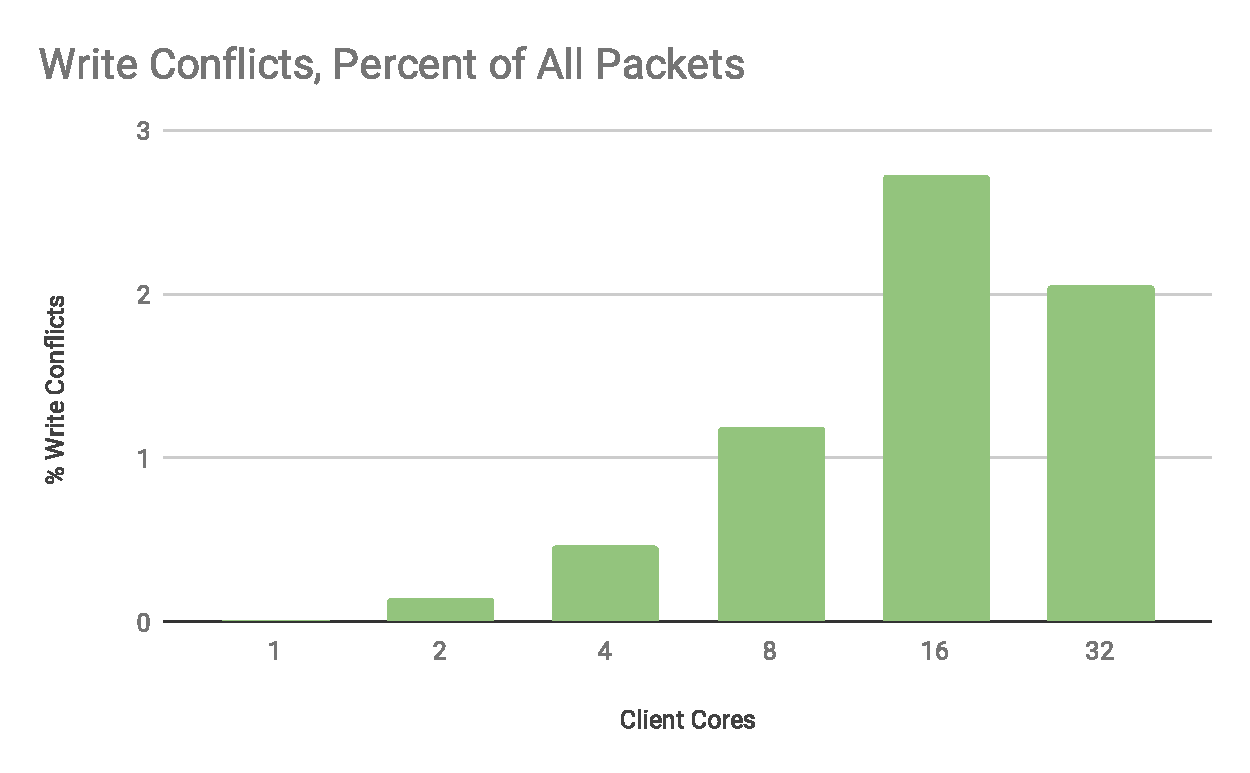
\includegraphics[width=0.45\textwidth]{fig/write_conflicts.pdf}
%    \caption{Clover write conflicts grow with the number of clients
%    (50\% write Zipf 0.99 distribution)\todo{redo with 64 cores and
%    writes only}}
%    \label{fig:conflicts}
%    \vskip -0.5em
%\end{figure}



%% The high level pitch about remote memory.
%Far memory projects typically have a remote CPU which is used to
%coordinate access to remote resources (cite all object systems). In a
%disaggregated system there is no remote CPU, therefore the coordination
%of reads and writes to remote locations must be done locally. For
%performance local caches of remote resources can be used to organize
%access to remote resources. For data structures which require
%consistency this creates a problem as stale caches can lead to data
%structure corruption.

